\documentclass[aspectratio=169]{beamer}
\usetheme{Madrid}
\usecolortheme{default}
\usepackage{tikz}
\usetikzlibrary{positioning, arrows.meta, shapes.geometric, calc}
\usepackage{listings}
\usepackage{xcolor}

\title{ACID-Compliant B+ Tree Database Engine}
\subtitle{Module A: Transaction Management \& Crash Recovery}
\author{CS 432 Databases - IIT Gandhinagar}
\date{\today}

\lstset{
  basicstyle=\ttfamily\footnotesize,
  keywordstyle=\color{blue},
  commentstyle=\color{gray},
  stringstyle=\color{red},
  showstringspaces=false,
  breaklines=true
}

\begin{document}

\frame{\titlepage}

\begin{frame}{Overview}
\tableofcontents
\end{frame}

\section{System Architecture}

\begin{frame}{System Architecture Overview}
\begin{center}
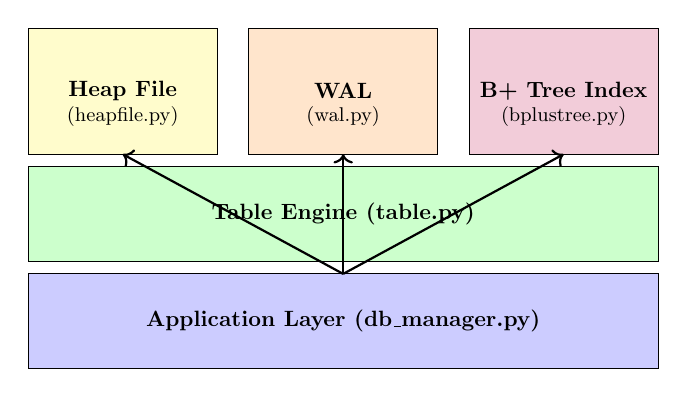
\begin{tikzpicture}[scale=0.8, every node/.style={scale=0.8}]
  % Layers
  \draw[fill=blue!20] (0,0) rectangle (10,1.5);
  \node at (5,0.75) {\textbf{Application Layer (db\_manager.py)}};
  
  \draw[fill=green!20] (0,1.7) rectangle (10,3.2);
  \node at (5,2.45) {\textbf{Table Engine (table.py)}};
  
  \draw[fill=yellow!20] (0,3.4) rectangle (3,5.4);
  \node at (1.5,4.4) {\textbf{Heap File}};
  \node at (1.5,4.0) {\small (heapfile.py)};
  
  \draw[fill=orange!20] (3.5,3.4) rectangle (6.5,5.4);
  \node at (5,4.4) {\textbf{WAL}};
  \node at (5,4.0) {\small (wal.py)};
  
  \draw[fill=purple!20] (7,3.4) rectangle (10,5.4);
  \node at (8.5,4.4) {\textbf{B+ Tree Index}};
  \node at (8.5,4.0) {\small (bplustree.py)};
  
  % Arrows
  \draw[->, thick] (5,1.5) -- (1.5,3.4);
  \draw[->, thick] (5,1.5) -- (5,3.4);
  \draw[->, thick] (5,1.5) -- (8.5,3.4);
\end{tikzpicture}
\end{center}
\end{frame}

\begin{frame}{Layered Storage Design}
\begin{block}{Why Separate Layers?}
\begin{itemize}
  \item \textbf{Heap File}: Durable row store with deterministic slot-based addressing
  \item \textbf{WAL}: Write-ahead log for crash safety and atomicity
  \item \textbf{B+ Tree}: Fast in-memory index (pk $\rightarrow$ slot\_id)
  \item \textbf{Metadata JSON}: Schema, allocator state, free list
\end{itemize}
\end{block}

\begin{alertblock}{Key Design Principle}
Heap file is the \textbf{source of truth}. Indexes are rebuilt from heap on startup.
\end{alertblock}
\end{frame}

\section{Storage Layer}

\begin{frame}[fragile]{Heap File: Fixed-Width Binary Storage}
\begin{block}{Record Layout}
\begin{lstlisting}[language=Python]
[tombstone: 1 byte]  # 0x01=alive, 0x00=deleted
for each column:
    [null_flag: 1 byte]  # 0x01=NULL, 0x00=present
    [data: N bytes]      # Type-specific encoding
\end{lstlisting}
\end{block}

\begin{itemize}
  \item \textbf{Fixed-width}: Enables O(1) slot addressing
  \item \textbf{Tombstone}: Logical deletion without physical compaction
  \item \textbf{Null flags}: Explicit NULL semantics
  \item \textbf{Type-aware encoding}: INT(4), FLOAT(8), BOOLEAN(1), CHAR/VARCHAR(N)
\end{itemize}
\end{frame}

\begin{frame}{Slot Allocation Strategy}
\begin{columns}
\column{0.5\textwidth}
\begin{block}{Two-Step Policy}
\begin{enumerate}
  \item Check free list (recycled slots)
  \item If empty, allocate next\_slot
\end{enumerate}
\end{block}

\begin{alertblock}{Benefits}
\begin{itemize}
  \item Prevents unbounded file growth
  \item Improves locality
  \item Stable slot IDs for WAL/indexes
\end{itemize}
\end{alertblock}

\column{0.5\textwidth}
\begin{center}
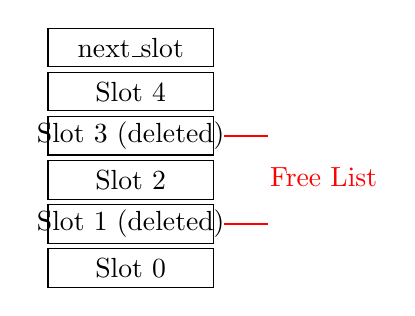
\begin{tikzpicture}[scale=0.7]
  \foreach \i in {0,1,2,3,4,5} {
    \draw (0,\i*0.8) rectangle (3,\i*0.8+0.7);
  }
  \node at (1.5,0.35) {Slot 0};
  \node at (1.5,1.15) {Slot 1 (deleted)};
  \node at (1.5,1.95) {Slot 2};
  \node at (1.5,2.75) {Slot 3 (deleted)};
  \node at (1.5,3.55) {Slot 4};
  \node at (1.5,4.35) {next\_slot};
  
  \draw[red, thick] (3.2,1.15) -- (4,1.15);
  \draw[red, thick] (3.2,2.75) -- (4,2.75);
  \node[red] at (5,2) {Free List};
\end{tikzpicture}
\end{center}
\end{columns}
\end{frame}

\section{Write-Ahead Logging}

\begin{frame}[fragile]{WAL Entry Structure}
\begin{block}{Binary Entry Format}
\begin{lstlisting}
[op: 1 byte]       # INSERT/UPDATE/DELETE/COMMIT_INTENT
[slot: 4 bytes]    # Heap slot ID
[txn_id: 4 bytes]  # Transaction ID (0=auto-commit)
[status: 1 byte]   # UNCOMMITTED/COMMITTED/ROLLEDBACK
[data: N bytes]    # Packed row bytes
\end{lstlisting}
\end{block}

\begin{itemize}
  \item \textbf{Fixed entry size}: HEADER(9) + status(1) + record\_size
  \item \textbf{O(1) status updates}: Direct seek to status byte
  \item \textbf{COMMIT\_INTENT}: Special marker indicating user's intent to commit
  \item \textbf{Idempotent replay}: Same entry can be applied multiple times
\end{itemize}
\end{frame}

\begin{frame}{WAL State Machine}
\begin{center}
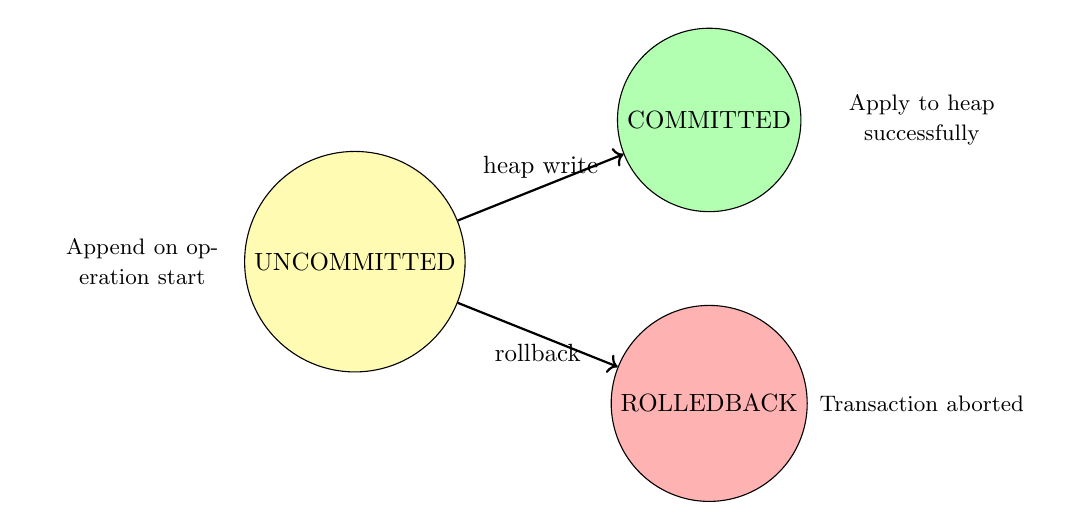
\begin{tikzpicture}[scale=0.9, every node/.style={scale=0.9}]
  \node[draw, circle, fill=yellow!30] (uncommitted) at (0,0) {UNCOMMITTED};
  \node[draw, circle, fill=green!30] (committed) at (5,2) {COMMITTED};
  \node[draw, circle, fill=red!30] (rolledback) at (5,-2) {ROLLEDBACK};
  
  \draw[->, thick] (uncommitted) -- node[above] {heap write} (committed);
  \draw[->, thick] (uncommitted) -- node[below] {rollback} (rolledback);
  
  \node[text width=3cm, align=center] at (-3,0) {\small Append on operation start};
  \node[text width=3cm, align=center] at (8,2) {\small Apply to heap successfully};
  \node[text width=3cm, align=center] at (8,-2) {\small Transaction aborted};
\end{tikzpicture}
\end{center}
\end{frame}

\section{Transaction Management}

\begin{frame}{Two Write Modes}
\begin{columns}
\column{0.5\textwidth}
\begin{block}{Auto-Commit (Thread-Safe)}
\begin{enumerate}
  \item Append WAL (uncommitted)
  \item Write to heap
  \item Mark WAL committed
  \item Update in-memory indexes
  \item Save metadata
\end{enumerate}
\textbf{Lock}: Per-table lock
\end{block}

\column{0.5\textwidth}
\begin{block}{Transaction Mode}
\begin{enumerate}
  \item Append WAL only (staged)
  \item Update indexes immediately (dirty reads)
  \item \textit{Heap untouched}
  \item On commit: apply all to heap
  \item On rollback: mark rolledback, rebuild indexes
\end{enumerate}
\textbf{Lock}: Single-threaded
\end{block}
\end{columns}

\vspace{0.5cm}
\begin{alertblock}{Key Insight}
Transaction staging updates indexes immediately for intra-transaction visibility, but keeps heap clean until commit.
\end{alertblock}
\end{frame}

\begin{frame}[fragile]{Transaction Lifecycle}
\begin{lstlisting}[language=Python]
txn = Transaction(users_table, orders_table)
txn.begin()  # Allocate unique txn_id

try:
    txn.insert(users_table, {"id": 1, "name": "Alice"})
    txn.insert(orders_table, {"id": 10, "user_id": 1})
    txn.commit()  # Apply all staged WAL entries to heap
except Exception:
    txn.rollback()  # Mark entries rolledback, rebuild index
    raise
\end{lstlisting}

\begin{itemize}
  \item \textbf{Atomicity}: All-or-nothing across multiple tables
  \item \textbf{Isolation}: Single-threaded execution per transaction
  \item \textbf{Durability}: WAL persisted before heap writes
\end{itemize}
\end{frame}

\begin{frame}{Commit Protocol with Intent Marker}
\begin{center}
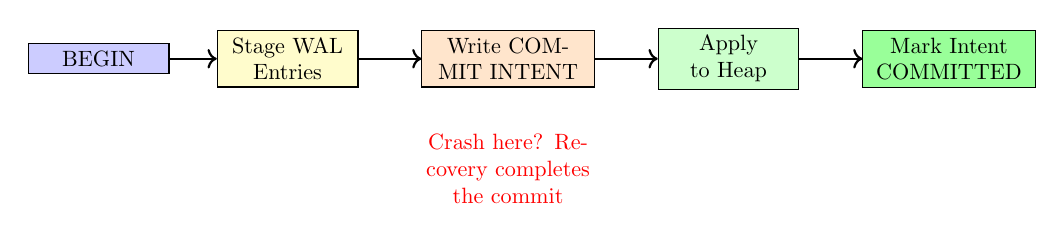
\begin{tikzpicture}[scale=0.8, every node/.style={scale=0.8}]
  \node[draw, rectangle, fill=blue!20, text width=2cm, align=center] (begin) at (0,0) {BEGIN};
  \node[draw, rectangle, fill=yellow!20, text width=2cm, align=center] (stage) at (3,0) {Stage WAL Entries};
  \node[draw, rectangle, fill=orange!20, text width=2.5cm, align=center] (intent) at (6.5,0) {Write COMMIT INTENT};
  \node[draw, rectangle, fill=green!20, text width=2cm, align=center] (apply) at (10,0) {Apply to Heap};
  \node[draw, rectangle, fill=green!40, text width=2.5cm, align=center] (mark) at (13.5,0) {Mark Intent COMMITTED};
  
  \draw[->, thick] (begin) -- (stage);
  \draw[->, thick] (stage) -- (intent);
  \draw[->, thick] (intent) -- (apply);
  \draw[->, thick] (apply) -- (mark);
  
  \node[text width=3cm, below=0.5cm of intent, red, align=center] {Crash here? Recovery completes the commit};
\end{tikzpicture}
\end{center}

\begin{alertblock}{Commit Intent Marker}
Critical for recovery: marks user's intent to commit. If crash occurs after this marker but before completion, recovery will finish the commit. Without this marker, uncommitted transaction entries are skipped during recovery.
\end{alertblock}
\end{frame}

\section{Crash Recovery}

\begin{frame}{Startup Recovery Pipeline}
\begin{enumerate}
  \item \textbf{Scan WAL}: Collect re-applicable entries
  \begin{itemize}
    \item UNCOMMITTED auto-commit entries (TXN\_AUTO)
    \item UNCOMMITTED entries belonging to transactions with COMMIT\_INTENT marker
  \end{itemize}
  \item \textbf{Apply to Heap}: Idempotent replay of intended commits
  \item \textbf{Skip}: COMMITTED (already applied) and ROLLEDBACK (intentionally discarded)
  \item \textbf{Truncate Corrupted Tail}: Handle partial writes
  \item \textbf{Rebuild Indexes}: From heap (source of truth)
  \item \textbf{Delete WAL}: Start fresh session
\end{enumerate}

\vspace{0.5cm}
\begin{block}{Deterministic Convergence}
System only replays operations the user intended to commit, ensuring ACID compliance.
\end{block}
\end{frame}

\begin{frame}{Recovery Decision Tree}
\begin{center}
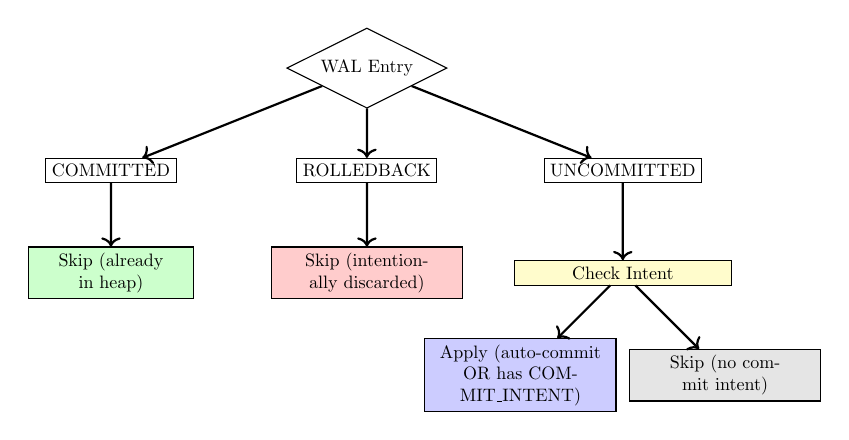
\begin{tikzpicture}[scale=0.65, every node/.style={scale=0.65}]
  \node[draw, diamond, aspect=2] (entry) at (0,0) {WAL Entry};
  
  \node[draw, rectangle] (committed) at (-5,-2) {COMMITTED};
  \node[draw, rectangle] (rolledback) at (0,-2) {ROLLEDBACK};
  \node[draw, rectangle] (uncommitted) at (5,-2) {UNCOMMITTED};
  
  \node[draw, rectangle, fill=green!20, text width=3cm, align=center] (skip1) at (-5,-4) {Skip (already in heap)};
  \node[draw, rectangle, fill=red!20, text width=3.5cm, align=center] (skip2) at (0,-4) {Skip (intentionally discarded)};
  \node[draw, rectangle, fill=yellow!20, text width=4cm, align=center] (check) at (5,-4) {Check Intent};
  
  \node[draw, rectangle, fill=blue!20, text width=3.5cm, align=center] (apply) at (3,-6) {Apply (auto-commit OR has COMMIT\_INTENT)};
  \node[draw, rectangle, fill=gray!20, text width=3.5cm, align=center] (skip3) at (7,-6) {Skip (no commit intent)};
  
  \draw[->, thick] (entry) -- (committed);
  \draw[->, thick] (entry) -- (rolledback);
  \draw[->, thick] (entry) -- (uncommitted);
  
  \draw[->, thick] (committed) -- (skip1);
  \draw[->, thick] (rolledback) -- (skip2);
  \draw[->, thick] (uncommitted) -- (check);
  
  \draw[->, thick] (check) -- (apply);
  \draw[->, thick] (check) -- (skip3);
\end{tikzpicture}
\end{center}
\end{frame}

\section{Consistency Mechanisms}

\begin{frame}{Foreign Key Constraints}
\begin{block}{Supported Actions}
\begin{itemize}
  \item \textbf{RESTRICT}: Prevent parent deletion if children exist
  \item \textbf{CASCADE}: Propagate delete/update to children
  \item \textbf{SET NULL}: Nullify child references
  \item \textbf{SET DEFAULT}: Set child references to default value
\end{itemize}
\end{block}

\begin{block}{Implementation}
\begin{itemize}
  \item Parent existence checks use indexed paths
  \item Child lookups via secondary indexes (efficient fan-out)
  \item Deep cascade chains supported
  \item Transaction-aware: cascades rollback with parent operation
\end{itemize}
\end{block}
\end{frame}

\begin{frame}{Secondary Indexes}
\begin{block}{Composite Key Design}
Secondary index stores: \texttt{(column\_value, pk)} in B+ tree
\end{block}

\begin{itemize}
  \item \textbf{Allows duplicates}: Multiple rows with same value
  \item \textbf{Deterministic retrieval}: PK ensures unique ordering
  \item \textbf{Efficient range scans}: Equality and range queries
  \item \textbf{FK acceleration}: Fast child lookups for cascades
\end{itemize}

\vspace{0.5cm}
\begin{exampleblock}{Example}
Index on \texttt{user\_id}: \texttt{(42, order\_1), (42, order\_5), (43, order\_2)}
\end{exampleblock}
\end{frame}

\section{Query Processing}

\begin{frame}{Condition Trees}
\begin{columns}
\column{0.5\textwidth}
\begin{block}{Expression Tree}
\begin{itemize}
  \item \textbf{Leaf}: column op value
  \item \textbf{AND/OR/NOT}: Combinators
  \item \textbf{Operators}: $=$, $\neq$, $<$, $>$, $\leq$, $\geq$, IN, BETWEEN, IS NULL
\end{itemize}
\end{block}

\column{0.5\textwidth}
\begin{center}
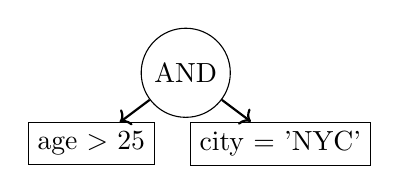
\begin{tikzpicture}[scale=0.6]
  \node[draw, circle] (and) at (0,0) {AND};
  \node[draw, rectangle] (age) at (-2,-1.5) {age $>$ 25};
  \node[draw, rectangle] (city) at (2,-1.5) {city = 'NYC'};
  
  \draw[->, thick] (and) -- (age);
  \draw[->, thick] (and) -- (city);
\end{tikzpicture}
\end{center}
\end{columns}

\vspace{0.5cm}
\begin{alertblock}{Conservative Optimization}
PK hints extracted only from safe AND branches. Final filtering always applied for correctness.
\end{alertblock}
\end{frame}

\begin{frame}{Join Strategies}
\begin{block}{Automatic Strategy Selection}
\begin{enumerate}
  \item \textbf{Index Nested-Loop}: Right join key is primary key
  \item \textbf{Secondary-Index Join}: Right join key has secondary index
  \item \textbf{Full Nested-Loop}: Fallback for unindexed predicates
\end{enumerate}
\end{block}

\begin{itemize}
  \item \textbf{LEFT JOIN}: Inject null-valued right columns when no match
  \item \textbf{Column hygiene}: Prefix right-table names on collision
  \item \textbf{WHERE filtering}: Applied after join merge
\end{itemize}
\end{frame}

\section{ACID Validation}

\begin{frame}{Atomicity Evidence}
\begin{block}{Transaction Rollback Scenarios}
\begin{itemize}
  \item Inserted records absent post-rollback
  \item Failure-injected branches show no partial visibility
  \item Cross-table inserts appear together or not at all
\end{itemize}
\end{block}

\begin{exampleblock}{Test Case 2: Mid-Transaction Failure}
\begin{itemize}
  \item Insert into users, products, orders
  \item Force exception before commit
  \item \textbf{Result}: All tables unchanged, no partial state
\end{itemize}
\end{exampleblock}
\end{frame}

\begin{frame}{Consistency Evidence}
\begin{block}{Schema \& Referential Integrity}
\begin{itemize}
  \item Invalid PK updates rejected
  \item FK checks prevent dangling references
  \item Cascade/SET NULL maintain referential closure
  \item Deep-chain cascades leave valid terminal state
\end{itemize}
\end{block}

\begin{exampleblock}{Test Case 3: 3-Table Order Transaction}
\begin{itemize}
  \item Atomic insert across users/products/orders
  \item FK violation attempts rejected
  \item Successful commit shows all constraints satisfied
\end{itemize}
\end{exampleblock}
\end{frame}

\begin{frame}{Isolation Evidence}
\begin{block}{Concurrency Control}
\begin{itemize}
  \item Auto-commit: Per-table lock serialization
  \item Stress workload: 50 high-contention updates
  \item \textbf{Result}: Aggregate flag sum = 50/50 (no lost updates)
\end{itemize}
\end{block}

\begin{exampleblock}{Test Case 4: Concurrent Transfers}
\begin{itemize}
  \item Original balance: 2,000,000
  \item 100+ concurrent transfer operations
  \item Final balance: 2,000,000
  \item \textbf{Invariant preserved}: No value creation or loss
\end{itemize}
\end{exampleblock}
\end{frame}

\begin{frame}{Durability Evidence}
\begin{block}{Persistence Across Restarts}
\begin{itemize}
  \item Committed rows available after close/reopen
  \item Deleted rows remain absent across restart
  \item Transaction-committed orders persist after reload
  \item WAL replay reconstructs consistent state
\end{itemize}
\end{block}

\begin{exampleblock}{Test Case 5: Restart Recovery}
\begin{itemize}
  \item Write committed, failed, and orphan staged work
  \item Simulate crash (close without cleanup)
  \item Restart and reload
  \item \textbf{Result}: Committed row persists, failed/orphan absent
\end{itemize}
\end{exampleblock}
\end{frame}

\section{Implementation Highlights}

\begin{frame}{File Organization}
\begin{columns}
\column{0.5\textwidth}
\begin{block}{Core System}
\begin{itemize}
  \item \texttt{table.py}: Table engine
  \item \texttt{heapfile.py}: Binary storage
  \item \texttt{wal.py}: Write-ahead log
  \item \texttt{transactions.py}: Txn coordinator
  \item \texttt{bplustree.py}: In-memory index
\end{itemize}
\end{block}

\column{0.5\textwidth}
\begin{block}{Constraints \& Query}
\begin{itemize}
  \item \texttt{column.py}: Schema validation
  \item \texttt{foreignkey.py}: Referential integrity
  \item \texttt{secondaryindex.py}: Non-PK indexes
  \item \texttt{conditions.py}: Expression trees
  \item \texttt{query.py}: Filter execution
  \item \texttt{join.py}: Join strategies
\end{itemize}
\end{block}
\end{columns}
\end{frame}

\begin{frame}{Design Rationale}
\begin{block}{Why Heap + WAL + In-Memory Index?}
\begin{itemize}
  \item \textbf{Heap}: Simple, deterministic slot-addressed persistence
  \item \textbf{WAL}: Operation-level idempotent replay
  \item \textbf{Index}: Reconstructed from committed row state
  \item \textbf{Trade-off}: Startup rebuild time vs. correctness simplicity
\end{itemize}
\end{block}

\begin{alertblock}{Alternative Rejected}
Direct B+ tree node serialization increases crash complexity (in-flight splits/merges).
\end{alertblock}
\end{frame}

\begin{frame}{Failure Modes Addressed}
\begin{enumerate}
  \item Crash after WAL append, before heap write
  \item Crash after heap write, before WAL status flip
  \item Crash during multi-entry transaction commit
  \item Truncated WAL tail (interrupted writes)
  \item Process restart with stale in-memory index
\end{enumerate}

\vspace{0.5cm}
\begin{block}{Recovery Guarantee}
For each failure class, startup replay + index rebuild converges to valid state.
\end{block}
\end{frame}

\section{Performance Characteristics}

\begin{frame}{Operation Complexity}
\begin{table}
\begin{tabular}{l|c|c}
\textbf{Operation} & \textbf{Time Complexity} & \textbf{Notes} \\
\hline
Insert & $O(\log n)$ & B+ tree insert + heap write \\
Find (PK) & $O(\log n)$ & B+ tree search \\
Update & $O(\log n)$ & Heap rewrite + index update \\
Delete & $O(\log n)$ & Tombstone + free list \\
Range Query & $O(\log n + k)$ & $k$ = result size \\
Secondary Lookup & $O(\log n + k)$ & Composite key scan \\
Cascade Delete & $O(m \cdot \log n)$ & $m$ = affected children \\
\hline
\end{tabular}
\end{table}

\vspace{0.3cm}
\begin{alertblock}{Startup Cost}
Index rebuild: $O(n \log n)$ where $n$ = total rows
\end{alertblock}
\end{frame}

\section{Testing \& Validation}

\begin{frame}{Validation Methodology}
\begin{block}{Behavioral Validation (Not Just Pass/Fail)}
\begin{itemize}
  \item \textbf{Atomicity}: Rollback leaves no partial state
  \item \textbf{Consistency}: FK violations rejected, cascades complete
  \item \textbf{Isolation}: Numeric invariants preserved under contention
  \item \textbf{Durability}: Committed data survives restart
\end{itemize}
\end{block}

\begin{alertblock}{Evidence-Based Approach}
Each test documents initial state, operation, and observed final state.
\end{alertblock}
\end{frame}

\section{Conclusion}

\begin{frame}{Key Achievements}
\begin{block}{From In-Memory B+ Tree to Transactional Engine}
\begin{itemize}
  \item \textbf{Persistent storage}: Fixed-width heap file with slot recycling
  \item \textbf{Crash safety}: Write-ahead logging with idempotent replay
  \item \textbf{ACID guarantees}: Atomicity, consistency, isolation, durability
  \item \textbf{Referential integrity}: Foreign keys with cascade actions
  \item \textbf{Query processing}: Condition trees, secondary indexes, joins
  \item \textbf{Validation}: 10+ usage scenarios + 5 explicit test cases
\end{itemize}
\end{block}

\begin{alertblock}{Core Principle}
Correctness through explicit data layout, operation sequencing, and failure-aware state transitions.
\end{alertblock}
\end{frame}

\end{document}